\section{Three Address Code}
We have implemented the three address code (3AC) using indirect triples. 
As stated by Aho et al. \cite{dragonbook}, this 
representation can help during the code optimization phase.
Indeed, the code optimizer can easily reorder the instructions without affecting
the triples themselves.

We generated the 3AC from the AST filtered by the type checker. 
To make it even easier to deal the instructions we chose to use
doubly-linked lists.

The following F code is represented in 3AC as depicted in Fig. 
\ref{fig:ind-trpl}:
\begin{verbatim}
fract a = [1|1];
fract b = [1|3] * a + [1|2];
\end{verbatim}

While traversing the AST we generate the three address code in a bottom up
fashion using \emph{only} synthesized attributes. This makes the three address
code generator intuitive.

\begin{figure}[H]
  \centering
  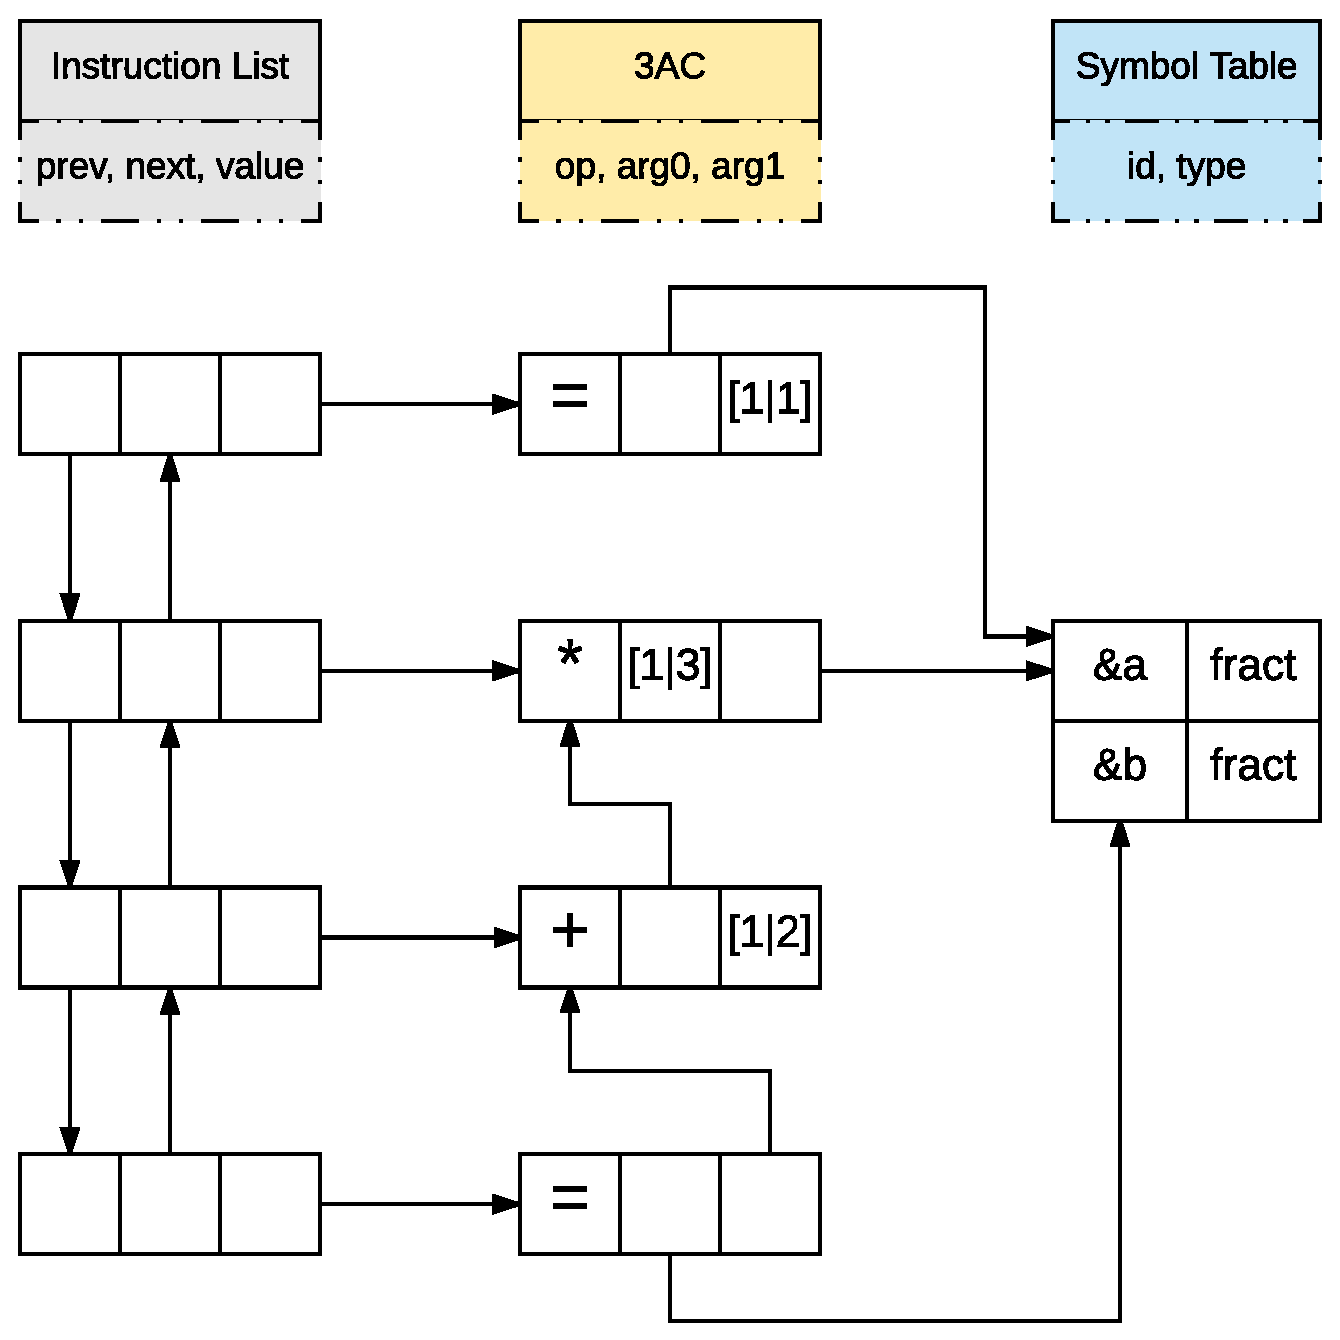
\includegraphics[width=.9\columnwidth]{img/eps/indirect_triples.eps}
  \caption{FAC - example of indirected triples.}
  \label{fig:ind-trpl}
\end{figure}
